\section{Introduction}
\label{sec:introduction}

% state the learning objective 
\par The objective of this laboratory assignment is to study a circuit containing only resistors and voltage/current sources, by determining all branch currents and all node voltages.
The scheme of the circuit we're going to analyse can be seen in figure~\ref{fig:Cir}.
\par \noindent On the first hand, in subsection~\ref{ssec:Mesh analysis}, a theoretical analysis of the circuit is
presented, based on the mesh analysis method, used to determine all branch currents. 
\par \noindent On the other hand, in subsection~\ref{ssec:Node analysis} we'll analyse the same circuit, using the node analysis method, in order to determine all node voltages.
\par \noindent To compare all these things, we present an error analysis in subsection~\ref{ssec:Error analysis}.
\par \noindent In section~\ref{sec:simulation}, the circuit is analysed by simulation, and the results are compared to the theoretical results obtained in
subsections~\ref{ssec:Mesh analysis} and~\ref{ssec:Node analysis}. 
\par \noindent The conclusions of this study are outlined in section~\ref{sec:conclusion}.

\begin{figure}[ht] \centering
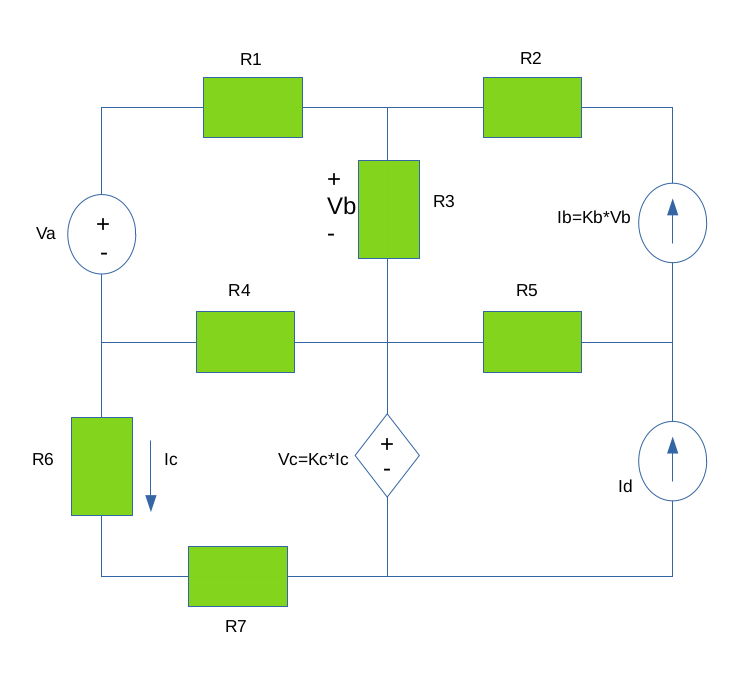
\includegraphics[width=0.8\linewidth]{Esquema_intro.png}
\caption{Circuit.}
\label{fig:Cir}
\end{figure}

